\documentclass{handout} 

% Rewritten from Equiprobable.tex for MathMethods exam 

\usepackage{handoutSetup}\usepackage{handoutShortcuts} 
 
\begin{document}

\handoutHeader

\begin{verbatimwrite}{\jobname.title}
Equiprobable Approximation to Bivariate Lognormal Returns
\end{verbatimwrite}

\handoutNameMake


\begin{verbatimwrite}{./body.tex}
  \newcommand{\sigAll}{\Sigma} % Chosen to be consistent with the Mathematica code, in which lower case sigma is a reserved variable
  
\newcommand{\scale}{x}
\provideboolean{riskyAltYN}\setboolean{riskyAltYN}{false}\newcommand{\ifriskyAlt}{\ifthenelse{\boolean{riskyAltYN}}}

This handout starts by defining a convenient notation to represent two rate-of-return shocks
that are distributed according to a multivariate lognormal that allows
for nonzero covariances.  It next presents a computationally
simple method for constructing a numerical approximation to that joint distribution.  The final
section uses both the numerical approximation, and more accurate (but enormously slower) standard numerical integration tools to assess the accuracy of the Campbell-Vicera analytical approximation to the solution to the optimal portfolio choice problem
described in \handoutA{Portfolio-Multi-CRRA}.  

\section{Statistical Theory}

Consider a set of two normally distributed risks
\begin{equation*}\begin{gathered}\begin{aligned}
   \ShkMeanOneLog_{2,t+1} & \sim & \mathcal{N}(-0.5 \sigAll^{2},\sigAll^{2})
\\ \ShkMeanOneLog_{1,t+1} & \sim & \mathcal{N}(-0.5 (\scale \sigAll)^{2},(\scale \sigAll)^{2})
\end{aligned}\end{gathered}\end{equation*}
which are statistically independent ($\ShkMeanOneLog_{1,t+1} \perp \ShkMeanOneLog_{2,t+1}$) even though the {\it scale} of shock 1's
{\it standard deviation} is determined by the proportionality factor
$\scale$ multiplied by the value of shock 2's standard deviation,
$\sigAll$.  (This permits us to increase or decrease the size of both risks
by changing $\sigAll$ and to adjust the relative size of risk 1 vs risk 2 by adjusting $\scale$.)

The $\ShkMeanOneLog$ are interpreted as the logarithms of level variables $\ShkMeanOne$, and the means of the log variables  have been chosen such that the expectations 
of the levels are independent of the size of the risk (cf.\ \MathFactsList).  That is, defining $\ShkMeanOne_{i} = \Ex_{t}[e^{\ShkMeanOneLog_{i,t+1}}]$ for $i \in \{1,2\}$:
\begin{equation}\begin{gathered}\begin{aligned}
   \ShkMeanOne_{i} \equiv     \Ex_{t}[\ShkMeanOne_{i,t+1}] & = & 1~\forall~i
\\ \log \Ex_{t}[\ShkMeanOne_{i,t+1}] & = & 0~\forall~i.
\end{aligned}\end{gathered}\end{equation}

From the first shock we can construct a log rate-of-return variable that can be represented equivalently in either of two ways:
\begin{equation}\begin{gathered}\begin{aligned}
    \ifriskyAlt{\riskyAlt_{1,t+1} = }{}      \risky_{1,t+1}  & = & \overbrace{\risky_{1}+0.5(\scale \sigAll)^{2}}^{\equiv \riskyAlt_{1}}+\ShkMeanOneLog_{1,t+1}
\\   & = & \underbrace{\riskyAlt_{1}-0.5(\scale \sigAll)^{2}}_{=\risky_{1}}+\underbrace{0.5(\scale \sigAll)^{2}+\ShkMeanOneLog_{1,t+1}}_{\equiv \ShkLogZeroLog_{1,t+1}}
\end{aligned}\end{gathered}\end{equation}
where $\ShkLogZeroLog_{1,t+1}~\sim~\mathcal{N}(0.,(\scale \sigAll)^{2})$; the notation for $\ShkLogZeroLog$ is motivated by the fact that the addition of the extra term cancels the nonzero mean of the original $\ShkMeanOneLog$.    Then
\begin{equation}\begin{gathered}\begin{aligned}
  \Risky_{1,t+1} \ifriskyAlt{= \acute{\Risky}_{1,t+1}}{} & \equiv & \ifriskyAlt{e^{\riskyAlt_{1,t+1}} =}{} e^{\risky_{1,t+1}}
\\ \Risky_{1} \ifriskyAlt{= \acute{\Risky}_{1} \equiv \Ex_{t}[\acute{\Risky}_{1,t+1}]}{} \equiv\Ex_{t}[\Risky_{1,t+1}] & = & \ifriskyAlt{e^{\riskyAlt_{1}+(\scale \sigAll)^{2}/2-(\scale \sigAll)^{2}/2}= e^{\riskyAlt_{1}} =}{}e^{\risky_{1}+(\scale \sigAll)^{2}/2} 
\\ \log \Ex_{t}[\Risky_{1,t+1}] \ifriskyAlt{= \log \Ex_{t}[\acute{\Risky}_{1,t+1}]}{} & = & \risky_{1}+(\scale \sigAll)^{2}/2 = \riskyAlt_{1} 
\end{aligned}\end{gathered}\end{equation}
where note to avoid confusion that $\riskyAlt_{1} \ifriskyAlt{= \log \Ex_{t}[\acute{\Risky}_{1,t+1}]}{} \neq \Ex_{t}[\ifriskyAlt{\acute}{}{{\risky}}_{1,t+1}]$ 
while $\log \Ex_{t}[\Risky_{1,t+1}] \neq \risky_{1}=\Ex_{t}[\risky_{1,t+1}]$.  

Using $\Ex_{t}[\ShkMeanOneLog_{2,t+1}] = -0.5 \sigAll^{2}$ and $\Ex_{t}[(\omega/\scale)\ShkMeanOneLog_{1,t+1}] = -0.5 ((\omega/\scale)\sigAll)^{2}$, we can by analogy define a second return
\begin{equation}\begin{gathered}\begin{aligned}
   \risky_{2,t+1} \ifriskyAlt{= \riskyAlt_{2,t+1}}{} & \equiv & \riskyAlt_{2}+\zeta + (\omega /\scale) \ShkMeanOneLog_{1,t+1} + \ShkMeanOneLog_{2,t+1} \label{eq:r2tp1CheckDef}
\\ & = & \riskyAlt_{2}+\zeta + (\omega /\scale) (\ShkLogZeroLog_{1,t+1}-0.5(\scale \sigAll)^{2}) + (\ShkLogZeroLog_{2,t+1}-0.5 \sigAll^{2})
\\ & = & \underbrace{\riskyAlt_{2}+\zeta -0.5 (\omega/\scale)(\scale \sigAll)^2-0.5 \sigAll^{2}}_{\risky_{2}}+(\omega /\scale) \ShkLogZeroLog_{t+1,1}  + \ShkLogZeroLog_{2,t+1} \label{eq:r2tp1Def}
\end{aligned}\end{gathered}\end{equation}
for some constants $\omega$ and $\zeta$.  

Since $(\omega/\scale)\ShkMeanOneLog_{1,t+1} $ is the only component of ${\risky}_{2,t+1}$ that is correlated with ${\risky}_{1,t+1}$,
\begin{equation*}\begin{gathered}\begin{aligned}
  \cov({\risky}_{1,t+1} ,{\risky}_{2,t+1})\ifriskyAlt{=  \cov(\riskyAlt_{1,t+1} ,\riskyAlt_{2,t+1})}{} & = & \cov({\risky}_{1,t+1} , (\omega/\scale){\risky}_{1,t+1} )
\\ & = & (\omega /\scale ) \underbrace{\cov({\risky}_{1,t+1} ,{\risky}_{1,t+1} )}_{=\scale^{2}\sigAll^{2}}
\\ & = & \omega \scale \sigAll^{2} \label{eq:Cov}
.
\end{aligned}\end{gathered}\end{equation*}

Thus, the parameter $\omega$ controls the covariance between the risky returns.  If we set $\omega = 0$ then $\risky_{1,t+1} \perp \risky_{2,t+1}$ (the returns are independent).

Next we want to find the value of $\zeta$ such that the expected level of the return is unaffected by $\sigAll$ (so
that we will be able to explore independently the distinct effects of the
components of each shock and their covariance):
\begin{equation}\begin{gathered}\begin{aligned}
  \Risky_{2} \ifriskyAlt{\equiv \acute{\Risky}_{2} \equiv \Ex_{t}[\acute{\Risky}_{2,t+1}]}{}\equiv  \Ex_{t}[\Risky_{2,t+1}] & = & e^{\riskyAlt_{2}}
\end{aligned}\end{gathered}\end{equation}
regardless of the values of $\scale$ and $\sigAll$.  Using \eqref{eq:r2tp1CheckDef}, we therefore need:
\begin{equation}\begin{gathered}\begin{aligned}
         \Ex_{t}[e^{\zeta+ (\omega/\scale)\ShkMeanOneLog_{1,t+1}  + \ShkMeanOneLog_{2,t+1}}] & = & 1
\\ \log  \Ex_{t}[e^{\zeta+ (\omega/\scale)\ShkMeanOneLog_{1,t+1}  + \ShkMeanOneLog_{2,t+1}}] & = & 0.
\end{aligned}\end{gathered}\end{equation}

Using standard facts about lognormals (cf. \MathFactsList), and for convenience 
defining $\hat{\omega}= (\sigAll/\scale) \omega$, we have 
\begin{equation}\begin{gathered}\begin{aligned}
  0. & = & \zeta - 0.5 \hat{\omega} \scale^{2} - 0.5 \sigAll^{2} + 0.5\hat{\omega}^{2}\scale^{2}+0.5  \sigAll^{2}
\\ & = & \zeta -0.5 \scale^{2} \hat{\omega}(1-\hat{\omega})
\\ \zeta & = & 0.5 (\hat{\omega}-\hat{\omega}^{2}) \scale^{2} = 0.5 (\omega \scale-\omega^{2}) \sigAll^{2}
\end{aligned}\end{gathered}\end{equation}
which means that we can rewrite \eqref{eq:r2tp1CheckDef} and \eqref{eq:r2tp1Def} directly as
\begin{equation*}\begin{gathered}\begin{aligned}
   \risky_{2,t+1} \ifriskyAlt{= \riskyAlt_{2,t+1}}{} & = & \riskyAlt_{2}+0.5 (\omega \scale-\omega^{2}) \sigAll^{2} + (\omega /\scale) \ShkMeanOneLog_{1,t+1} + \ShkMeanOneLog_{2,t+1} 
%\\ & = & \riskyAlt_{2}+0.5 (\omega \scale-\omega^{2}) \sigAll^{2} + (\omega /\scale) (\ShkLogZeroLog_{1,t+1}+0.5(\scale \sigAll)^{2}) + (\ShkLogZeroLog_{2,t+1}+0.5 \sigAll^{2})
\\ & = & \riskyAlt_{2}+0.5 (\omega \scale-\omega^{2}) \sigAll^{2} -0.5 (\omega/\scale)(\scale \sigAll)^2-0.5 \sigAll^{2}+(\omega /\scale) \ShkLogZeroLog_{t+1,1}  + \ShkLogZeroLog_{2,t+1} 
\\ & = & \riskyAlt_{2}+0.5 \omega \scale \sigAll^{2} -0.5 \omega\scale \sigAll^2 - 0.5 \omega^{2} \sigAll^{2}-0.5 \sigAll^{2}+(\omega /\scale) \ShkLogZeroLog_{t+1,1}  + \ShkLogZeroLog_{2,t+1} 
\\ & = & \underbrace{\riskyAlt_{2} - (1+\omega^{2})0.5 \sigAll^{2}}_{\risky_{2}}+(\omega /\scale) \ShkLogZeroLog_{t+1,1}  + \ShkLogZeroLog_{2,t+1} 
.
\end{aligned}\end{gathered}\end{equation*}


Hence, from the independent mean-one lognormally distributed shocks
$\ShkMeanOne_{1}$ and $\ShkMeanOne_{2}$, we have constructed a pair of
jointly lognormally distributed shocks whose covariance is controlled
by the parameter $\omega$, whose relative and absolute variances are
controlled by the parameters $\scale$ and $\sigAll$, and whose means
are $\risky_{1}$ and $\risky_{2}$.

To sum up, the process can be described in either of two ways:
\begin{equation*}
 \left(\begin{array}{c}\risky_{1,t+1} \\ \risky_{2,t+1} \end{array}\right) \sim \left(\begin{array}{c}\mathcal{N}(\risky_{1},\scale^{2} \sigAll^{2}) \\ \mathcal{N}(\risky_{2}, \phantom{\scale^{2}} \sigAll^{2}) \end{array}\right) = \left(\begin{array}{c}\mathcal{N}(\riskyAlt_{1}-0.5(\scale\sigAll)^{2},\scale^{2} \sigAll^{2}) \\ \mathcal{N}(\riskyAlt_{2} - (1+\omega^{2})0.5 \sigAll^{2}, \sigAll^{2}) \end{array}\right) 
\end{equation*}
with covariance matrix
\begin{equation}
\left(\begin{array}{ccc}\sigma_1^2 & \sigma_{12} \\ \sigma_{12}& \sigma_2^2\end{array}\right) \equiv \left(\begin{array}{ccc}(\scale \sigAll)^2 & \scale \omega \sigAll^{2} \\ \scale \omega \sigAll^{2}  & (\omega^{2}+1)\sigAll^{2}\end{array}\right) \label{eq:CovMat}
\end{equation}
where a final useful result that follows from \eqref{eq:CovMat} and \eqref{eq:Cov} is 
\begin{equation}\begin{gathered}\begin{aligned}
 \text{corr}({\risky}_{1,t+1} ,{\risky}_{2,t+1}) \ifriskyAlt{= \text{corr}(\riskyAlt_{1,t+1} ,\riskyAlt_{2,t+1})}{} & \equiv & \cov({\risky}_{1,t+1} ,{\risky}_{2,t+1})/\sigma_{1}\sigma_{2}
\\ & = & \omega/(1+\omega^{2})^{0.5} .
\end{aligned}\end{gathered}\end{equation}

\section{Computational Theory}

To reduce clutter, define $\tilde{\Risky}_{i}=\Risky_{i,t+1}$ and interpret $\Ex$ as $\Ex_{t}[]$, so that we can write the expectation of some function $\hFunc$ that depends on the realization of
the return shocks as:
\begin{equation}\begin{gathered}\begin{aligned}
  \Ex[\hFunc(\tilde{\Risky}_{1},\tilde{\Risky}_{2})] & = & \int_{\underline{{\Risky}}_{1}}^{\bar{\Risky}_{1}}\int_{\underline{\Risky}_{2}}^{\bar{\Risky}_{2}} \hFunc(\tilde{\Risky}_{1},\tilde{\Risky}_{2}) d\FFunc(\tilde{\Risky}_{1},\tilde{\Risky}_{2})
\end{aligned}\end{gathered}\end{equation}
where $\FFunc(\tilde{\Risky}_{1},\tilde{\Risky}_{2})$ is the cumulative distribution
function for a multivariate lognormal with the covariance matrix defined by \eqref{eq:CovMat}.\footnote{Under the lognormal assumption, $\underline{\tilde{\Risky}}_{i}=0$ and $\bar{\Risky}_{i}=\infty$ for both shocks $i \in \{1,2\}$.}  Standard numerical computation software can compute this
double integral, but at such a slow speed as to be unusable for many purposes.
Computation of the expectation can be massively speeded up by
advance construction of a numerical approximation to
$\FFunc(\tilde{\Risky}_{1},\tilde{\Risky}_{2})$.

Such approximations often take the approach of replacing the distribution function
with a discretized approximation to it; appropriate weights $w[i,j]$ are attached to
each of a finite set of points indexed by $i$ and $j$, and 
the approximation to the integral is given by:
\begin{equation}\begin{gathered}\begin{aligned}
  \Ex[\hFunc(\tilde{\Risky}_{1},\tilde{\Risky}_{2})] & \approx & \sum_{i=1}^{n}\sum_{j=1}^{m} \hFunc(\hat{\Risky}_{1}[i,j],\hat{\Risky}_{2}[i,j])w[i,j]  \label{eq:wtdAvg}
\end{aligned}\end{gathered}\end{equation}
where various methods are used for constructing the weights $w[i,j]$ and the nodes (corresponding to the $\{i,j\}$ pairs).  The matrices $\hat{\Risky}_{1}$ and $\hat{\Risky}_{2}$ contain the conditional mean values of $\tilde{\Risky}_{1}$ and $\tilde{\Risky}_{2}$ associated with each of the regions.

Perhaps the most popular such method is Gauss-Hermite interpolation
(see \cite{judd:book} for an exposition, or \cite{kopecky2010finite}
for a recent candidate for a better choice).  Here, we will pursue a
particularly simple and intuitive alternative: Equiprobable discretization.  In
this method, $m=n$ and boundaries on the joint CDF are determined in
such a way as to divide up the total probability mass into submasses
of equal size (each of which therefore has a mass of $n^{-2}$).  This
is conceptually easier if we represent the underlying shocks as
statistically independent, as with $\ShkMeanOne_{1}$ and
$\ShkMeanOne_{2}$ above; in that case, each submass is a square region
in the $\ShkMeanOne_{1}$ and $\ShkMeanOne_{2}$ grid.  We then compute
the average value of $\ShkMeanOne_{1}$ and $\ShkMeanOne_{2}$ {\it
  conditional} on their being located in each of the subdivisions of
the range of the CDF.  Since $\ShkMeanOne_{1}$ and $\ShkMeanOne_{2}$
are IID, the representation of the approximating summation is even
simpler than \eqref{eq:wtdAvg}:
\begin{equation*}\begin{gathered}\begin{aligned}
  \Ex\left[\hFunc\left(\tilde{\Risky}_{1},\tilde{\Risky}_{2})\right)\right] & \approx & n^{-2} \sum_{i=1}^{n}\sum_{j=1}^{n} \hFunc\left(\Risky_{1}(\hat{\ShkMeanOne}_{1}[i],\hat{\ShkMeanOne}_{2}[j]),\Risky_{2}(\hat{\ShkMeanOne}_{1}[i],\hat{\ShkMeanOne}_{2}[j]))\right) \label{eq:wtdAvgMod}
\end{aligned}\end{gathered}\end{equation*}
where $\Risky_{i}(\ShkMeanOne_{1},\ShkMeanOne_{2})$ are the (linear) functions relating the return shocks to the IID shocks.


\section{Computational Results}
\begin{figure}
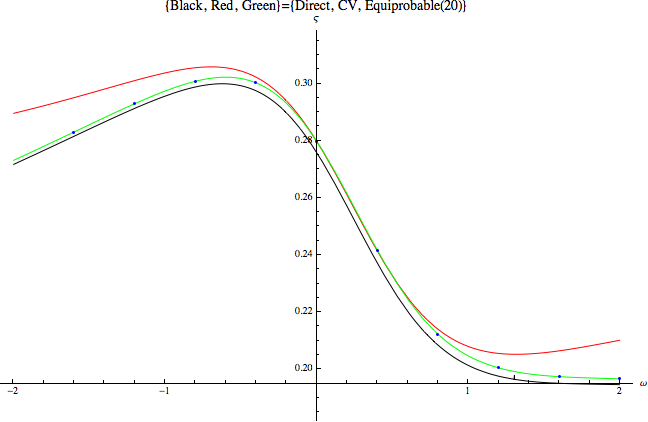
\includegraphics[width=6in]{../Figures/ShareVsCovByMethod}
\caption{Portfolio Share By Method as a Function of $\omega$}\label{fig:ShareVsCovByMethod}
\end{figure}

Figure~\ref{fig:ShareVsCovByMethod} compares the computed optimal portfolio share for a numerical solution 
using the built-in numerical optimizer and maximization functions (the lowest, black, locus), the Campbell-Viceira solution (the highest, red locus)
and an equiprobable approximation using 20 approximation points (green, middle) as well as the solution using the equiprobable approximation
at an evenly-spaced grid of points (blue dots).  

Careful examination indicates that the numerical approximation is quite close to the full numerical solution, while the CV approximation diverges substantially from the numerical answer.  The tradeoff is that the 
equiprobable solution is about 2000 times slower than the CV approximation, while the direct solution is more than 100 times slower
than the equiprobable solution.  Depending on the requirements of the problem being examined, these differences in 
efficiency can make a tremendous difference in the feasibility of a research project.\footnote{Details can be found in the {\it Mathematica} notebook associated withthis handout.}

\end{verbatimwrite}

\centerline{\href{\publec}{\texttt{\publec}}}

\newcommand{\dir}{/Volumes/Data/Courses/Choice/LectureNotes/MathFacts/Handouts}

\input makePostHandoutsStart.tex

\newcommand{\hBoth}[1]{\href{\toDir/#1.pdf}{[pdf]}\href{\toDir/#1}{[html]}}
\begin{entry}
\input ../../Index/MathFactsList.tex
\input ../../Index/Aggregation.tex
\end{entry}

\write18{chmod a+x makePostHandouts.sh}
\write18{touch makePostHandouts.sh ; mv makePostHandouts.sh /Volumes/Data/Courses/Choice/LectureNotes/MathFacts/makePostMathFacts/makePostHandouts604.sh}



\input handoutBibMake.tex

\end{document}
